\section{Phase Space Definition}
\label{sec:FidSel}

The unfolded differential cross-sections are measured in a phase space within the acceptance of the detector. This section summarizes the selections defining the fiducial phase space of the analysis.

\subsection{Fiducial Volume}
\label{subsec:FidVol} 

The fiducial phase space consists of events with $pp\rightarrow ZZjj \rightarrow 4\ell jj ~(\ell = e,~\mu)$ with four centrally produced prompt-leptons and two jets with large rapidity gap as motivated by section \ref{sec:EWKPheno}. The fiducial phase space does not contain any leptons from the decays of unstable taus. Both particle-level electrons and muons are required to be at a dressed level. Dressed leptons in MC generators are constructed by adding the four-momenta of nearby photons emitted by the lepton within a cone size of $\Delta R < 0.1$. 

To ensure the selected events fall within detector acceptance, several kinematic cuts summarized in Table \ref{tab:FidObjectCut} are applied individually to the muons, electrons, and jets before defining the event quadruplet and dijet. Each electrons are required to have $p_{T} > 7$ GeV and $|\eta| < 2.47$, whereas the muons satisfy $p_{T} > 5$ GeV and $|\eta| < 2.7$. Lepton quadruplets are formed by requiring two same-flavor, SF-OC lepton pairs, with leading and sub-leading lepton $p_{T}>20$ GeV and angular separation between any two leptons to satisfy $\Delta R > 0.05$. Additionally, the invariant mass of any SF-OC lepton pair is required to satisfy $m_{\ell \ell } > 5$ GeV to suppress the contamination from lower resonance backgrounds. Based on these requirements, the quadruplets can be of the following three types:

\begin{itemize}
\item{$4e$: events with two $e^{+}e^{-}$ pairs.}
\item{$4\mu$: events with two $\mu^{+}\mu^{-}$ pairs.}
\item{$2e2\mu$ or $2\mu2e$: events where one of the pair is $e^{+}e^{-}$ and other is $\mu^{+}\mu^{-}$}
\end{itemize}

In any event with more than two SF-OC lepton pairs, the quadruplet is formed by choosing the two pairs that minimize the distance to the $Z$ resonance pole. Once the quadruplet is formed, the leading-lepton pair is defined as the one with a higher absolute rapidity value, i.e., $|y_{ij}|$. Finally, an additional criterion of $m_{4\ell} > 130$ GeV is imposed on the invariant mass of the quadruplet. 

Similarly, the di-jet in the fiducial phase space are also constructed from the leading-dressed jets with opposite sign of pseudo-rapidity ($\eta$) to imitate the detector-level VBS di-jet production where jets are reconstructed on the opposite side of the detector. The jets are required to satisfy $|n| < 4.5$, $p_{T,~leading~jet} > 40$ GeV, and $p_{T,~sub-leading~jet} > 30$ GeV. The di-jet is required to have a large rapidity separation of $|\Delta y_{jj}| > 2$ and $m_{jj} > 300$ GeV to resemble dijet produced in electroweak $ZZjj$ production. Table \ref{tab:QuadDijetFidCut} summarizes the requirements to select quadruplet and the di-jet in an event.

\begin{table}[ht]
	\centering
	\caption{Details of the kinematic pre-selection applied to the dressed baseline electrons, muons, and jets.
	\label{tab:FidObjectCut}}
	\begin{tabular}{|| l || c | c | c ||}
		\hline
		Selections 		& Electrons 			& 		Muons		 & 			Jets 			\\
		\hline\hline
		$\Pt~$ 			& $> 7$ GeV 			& 		$ >5$ GeV  	 & 		$>30$GeV 		\\
		\hline 
		$|\eta|$			&  $< 2.47	$			& 		$ < 2.7 $		 &		$ < 4.5$ 			\\
		\hline
	\end{tabular}
\end{table}				
	
\begin{table}[ht]
	\caption{Details of the selections applied to form a quadruplet and a dijet selection in the fiducial volume. 
	\label{tab:QuadDijetFidCut}}
	\begin{tabular}{|| l || c ||}
		\hline
		Selections 				&	 		Cut	\\
		\hline\hline
		Lepton Kinematics 		& $P_{T,~leading~lepton} > 20 $ GeV\\
				 				& $P_{T,~sub-leading~lepton} > 20 $ GeV\\
		\hline 
		Pair Requirement 		& $\Delta R_{\ell i,\ell	 j} > 0.05 $\\
		 						& SF-OC with $\mll > 5$ GeV\\
		\hline
		Quadruplet Requirement	& $2$ pair candidates with smallest $|\mOneTwo	- m_{Z} | + |\mThreeFour	- m_{Z} |$	\\
								& Leading pair: pair with highest $|y_{ij}|$\\
								& Sub-leading pair: pair with lowest $|y_{ij}|$\\
								& $\mFourL > 130 $ GeV\\
		\hline
		Di-jet Requirement		& $p_{T,~leading~jet} > 40$ GeV	\\
								& $|\Delta y_{jj}| > 2 $ \\	
								& $m_{jj} > 300$ GeV	\\
		\hline
	\end{tabular}
\end{table}

\subsection{Signal Region}
\label{subsec:SignalRegion}
The signal region of the analysis is defined based on the centrality ($\zeta$) of the di-$Z$boson production in an event. Centrality depends on the rapidity of the quadruplet and the rapidity of the dijet as:
	\begin{equation}
		\zeta~=~\frac{|y_{quadruplet}~-~ 0.5*(y_{leading~jet}~+~y_{sub-leading~jet})| }{|y_{leading~jet}~-~y_{sub-leading~jet}|}
		\label{eq:centr}
	\end{equation}

Figure \ref{fig:centrality_a} shows the distribution of centrality in MC for the three main production modes of $ZZjj$. The chosen cut value on the $ZZjj$ centrality maximizes the significance of the EWK component over the inclusive $qq$ and $gg$-initiated QCD production (defined as $s=\frac{N_{EWK}}{\sqrt{N_{QCD}^{(qq)}+N_{QCD}^{(gg)}}}$) while maintaining a good selection efficiency of EWK events. The second distribution in \ref{fig:centrality_b} shows the efficiency and significance for various cut values.  

A VBS-enhanced signal region is defined based on events with a quadruplet, a dijet, and $\zeta<0.4$. The low value of the centrality and the requirements for a signal dijet ensures that the events in this signal region originate in a more significant fraction from the electroweak production of $ZZjj$. A VBS Suppressed control region is also defined based on events with a quadruplet, a dijet, and $\zeta>0.4$. These events mainly originate from the QCD production of ZZjj and are used to optimize the analysis strategies.

\begin{figure}[ht]
\begin{subfigure}{.48\textwidth}
  \centering
  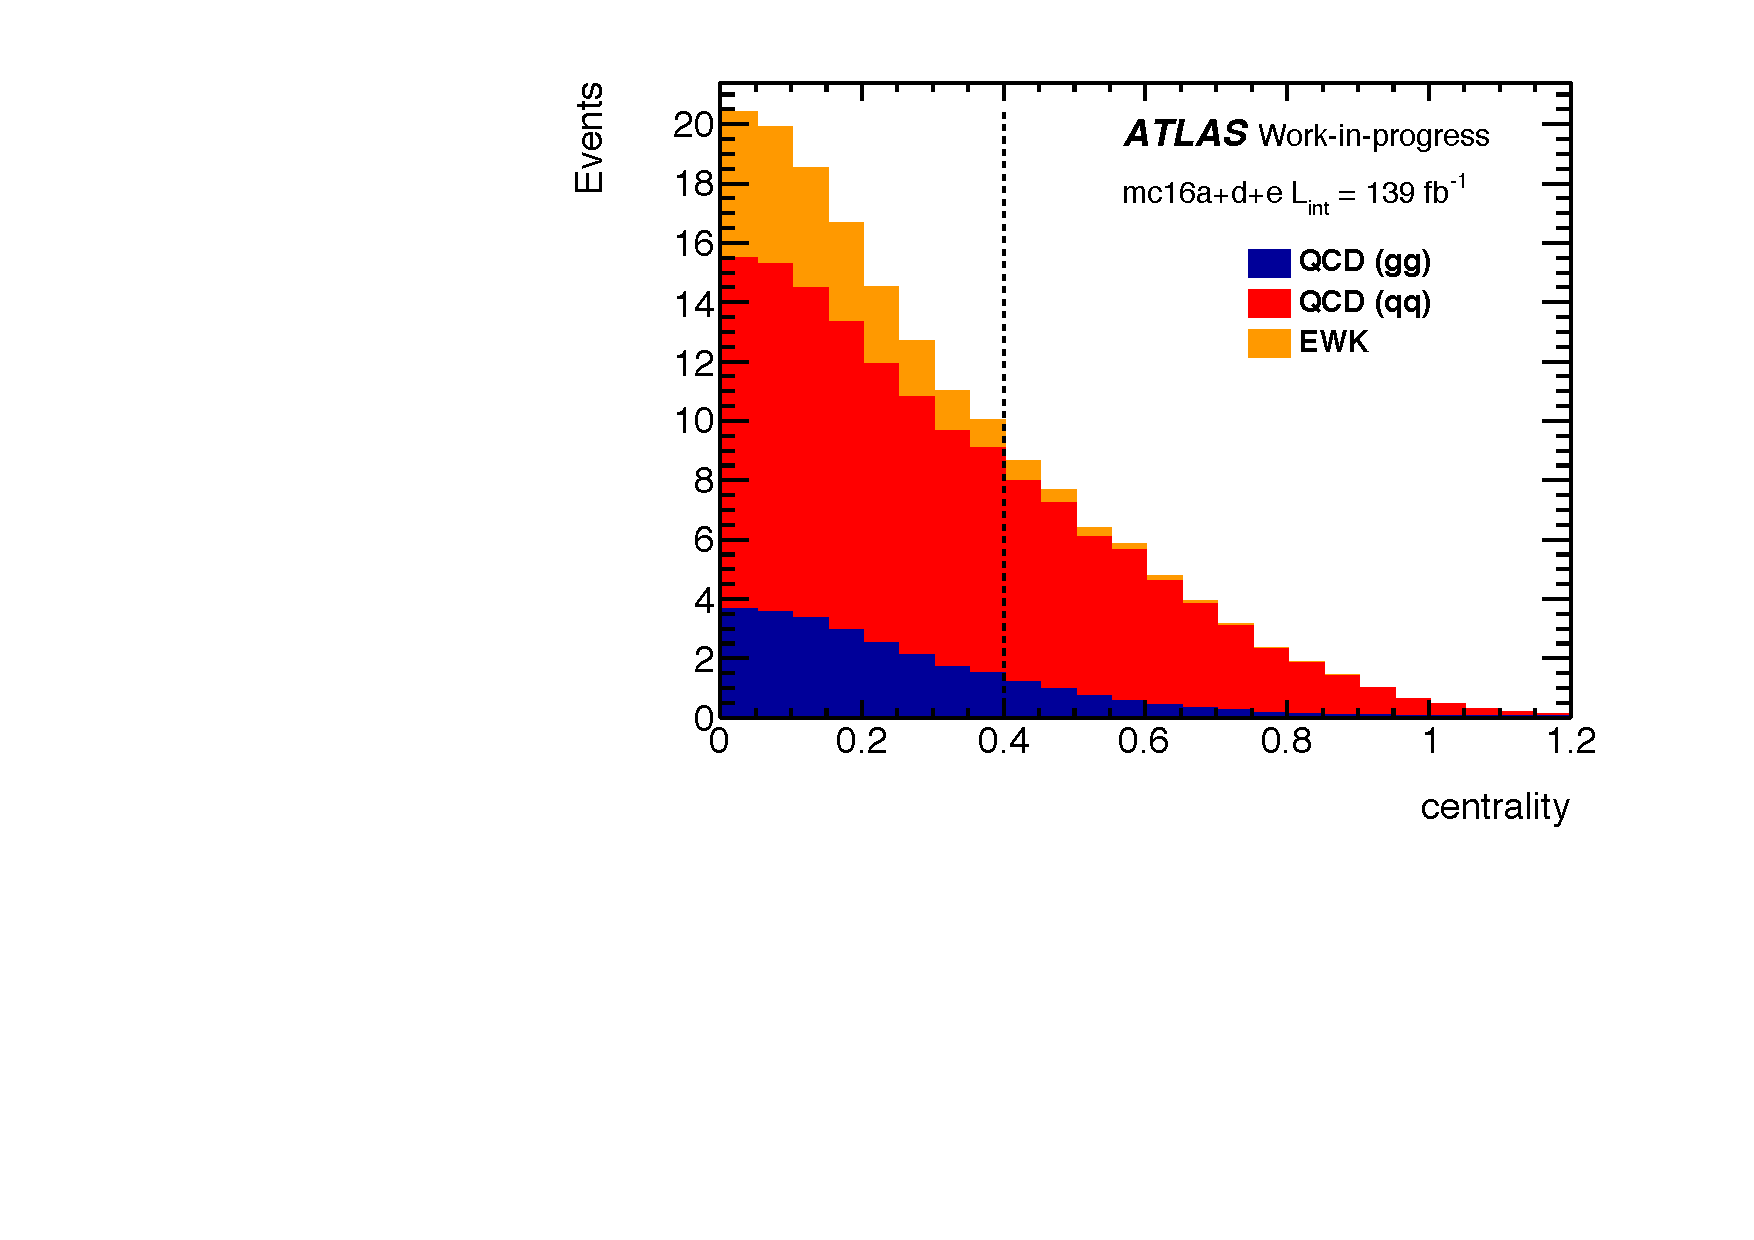
\includegraphics[width=.8\linewidth]{figures/AnalysisOverview/centrality_Dist.pdf}  
  \caption{Yields of EWK(red) and QCD (parton initiated in blue, gg-loop initiated in green) ZZjj production as a function of centrality.}
  \label{fig:centrality_a}
\end{subfigure}
\begin{subfigure}{.48\textwidth}
  \centering
  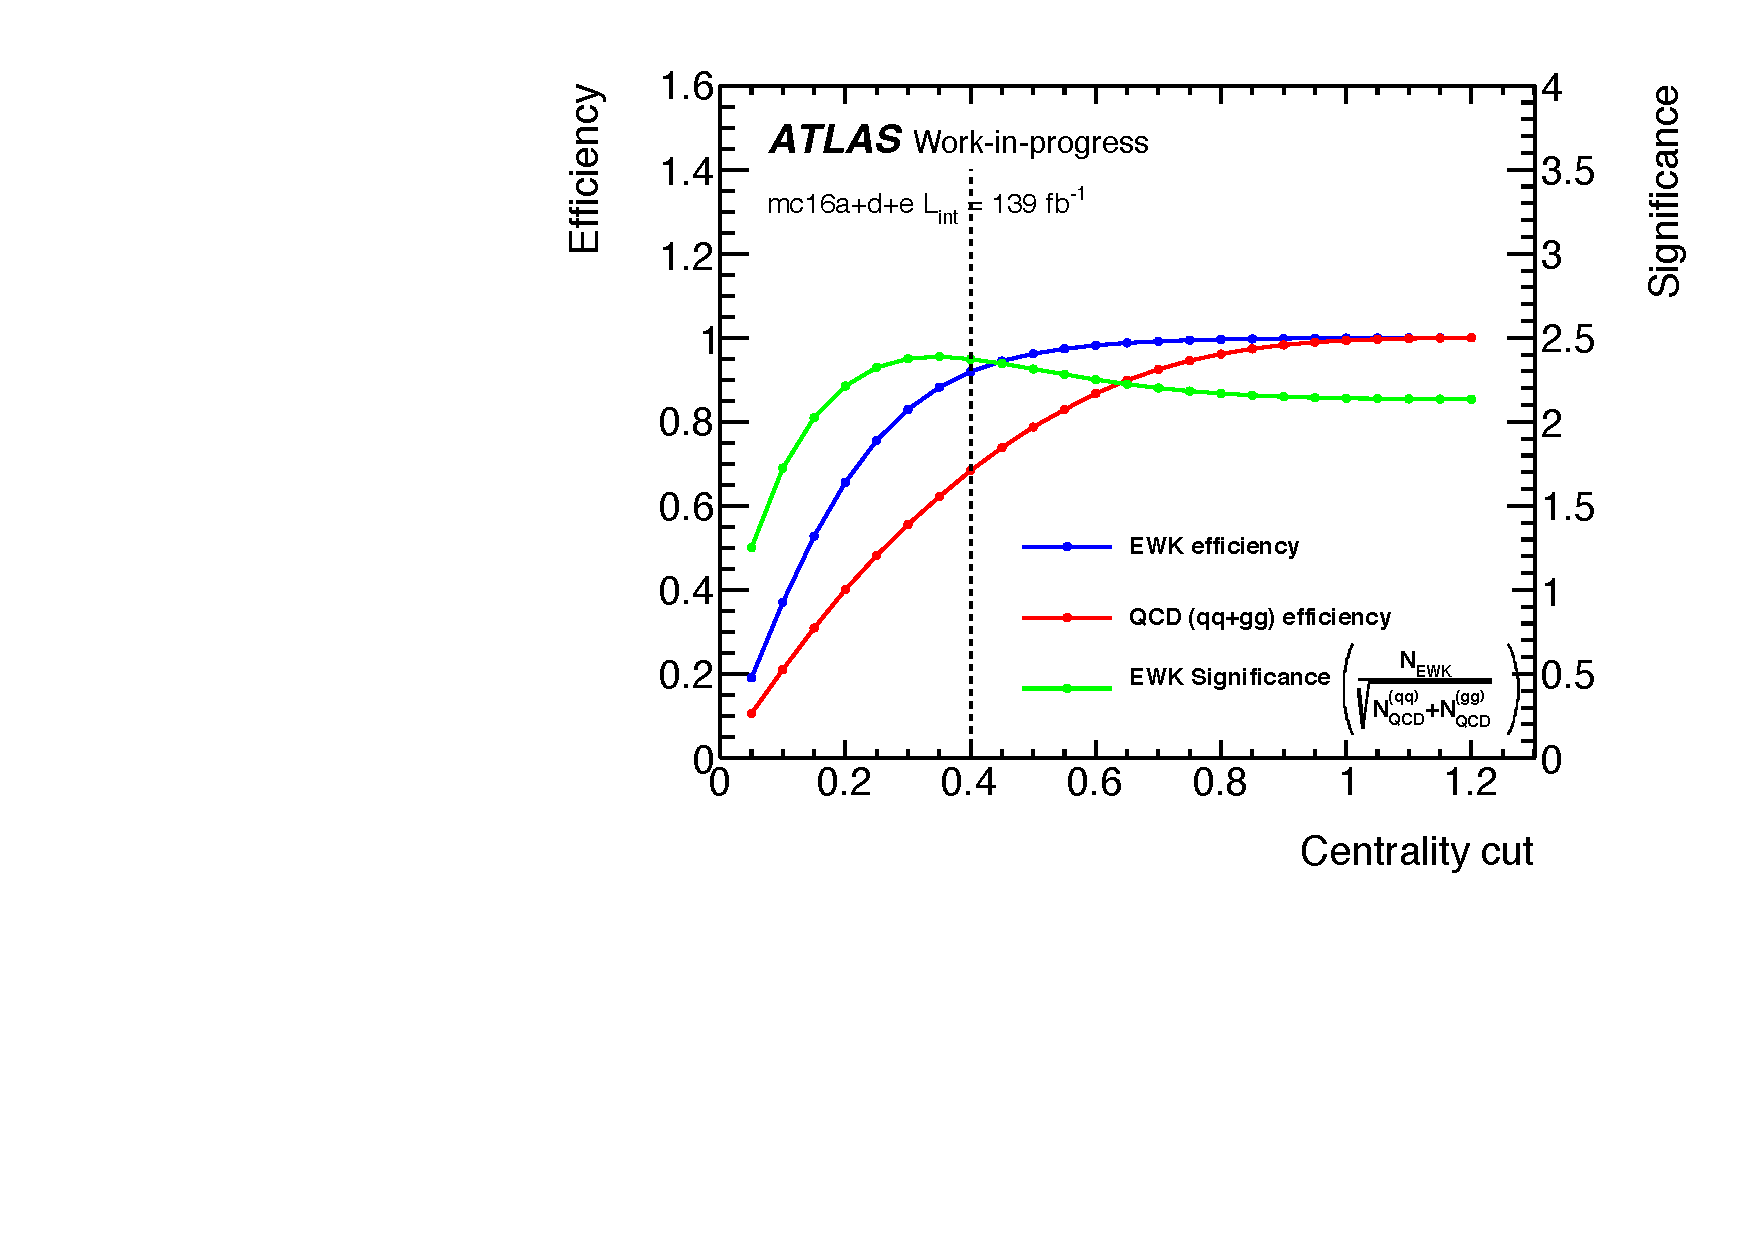
\includegraphics[width=.8\linewidth]{figures/AnalysisOverview/centrality_Cut.pdf}  \\
  \caption{Selection efficiency (EWK in blue, QCD in red) and EWK significance (green) for different centrality cut values. The dashed line highlights the selected cut values of 0.4.}
  \label{fig:centrality_b}
\end{subfigure}

\end{figure}
